              
\documentclass[12pt]{article}
 \usepackage[margin=1in]{geometry} 
\usepackage{amsmath,amsthm,amssymb,amsfonts, graphicx, tikz, placeins, algorithmicx, hyperref}
\usepackage[ruled, linesnumbered]{algorithm2e}
\usetikzlibrary{positioning}
 
\newcommand{\N}{\mathbb{N}}
\newcommand{\Z}{\mathbb{Z}}
 
%\newenvironment{problem}[2][Problem]{\begin{trivlist}
%\item[\hskip \labelsep {\bfseries #1}\hskip \labelsep {\bfseries #2.}]}{\end{trivlist}}
%If you want to title your bold things something different just make another thing exactly like this but replace "problem" with the name of the thing you want, like theorem or lemma or whatever
 
\begin{document}
 
%\renewcommand{\qedsymbol}{\filledbox}
%Good resources for looking up how to do stuff:
%Binary operators: http://www.access2science.com/latex/Binary.html
%General help: http://en.wikibooks.org/wiki/LaTeX/Mathematics
%Or just google stuff
 
\title{Homework 2}
\author{Selma Wanna \\ SLW3429 \\ slwanna@utexas.edu} 
\maketitle
 
\section{Introduction}

Homework 2 focuses on leveraging Independent Component Analysis (ICA) in conjunction with Gradient Descent to solve the Blind Signal Separation (BSS) problem.
\bigbreak
\noindent
BSS involves separating source signals after they have been altered by an unknown mixing matrix: A. In our assignment, five source signals (as sound waves) are provided with 44000 time samples. We then mix these sounds with a randomly generated: A then use ICA to resolve the original signals from the sound mixture.  
\bigbreak
\noindent
Given a \(s\) by \(t\) matrix: \(S\), of original sound signals and a \(n\) by \(t\) matrix: \(A\), which mixes the original signals by means of randomly generated coefficients, the mixed signal matrix: \(X\) is determined by the equation below. 
\begin{equation}
    X = AS
\end{equation}
\bigbreak
\noindent
In order to recover the original signal matrix \(S\), we must approximate the reconstruction matrix \(W\) as shown below.
\begin{equation}
    \hat{S}=WX
\end{equation}
From the inspection of equations (1) and (2), \(W\) should be approximated as \(A^{-1}\); however, because \(A\) is an unknown in this problem, ICA is selected to determine \(W\). 
\bigbreak
\noindent
The first step in ICA is recognizing that the source signals that make up \(S\) are independent from each other. Thus, we can treat the resulting mixed signal's pdf as follows.

\begin{equation}
    p(x)=\prod_{i=1}^{n}p_{s}(w_{i}^{T}x\cdot \left | W \right |)
\end{equation}
\bigbreak
\noindent
In Equation (3), \(w_{i}^{T}\) refers to the rows of matrix \(W\) as shown in Fig. 1 on the next page. Equation (4) demonstrates how the \(i\)-th source signal can be determined by leveraging the information in the rows of \(W\). 

\begin{figure}[h] % replace 't' with 'b' to force it to be on the bottom
  \centering
  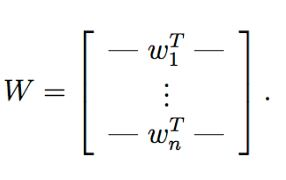
\includegraphics[width = 0.2\linewidth]{yeesh.JPG}
  \caption{Description of the Reconstruction Matrix: W}
\end{figure}

\begin{equation}
    s_{i}=w_{i}^{T}x
\end{equation}
\bigbreak
\noindent
Because the pdf: \(p_{s}\) in Equation (3) is unknown, a cdf commonly used in audio applications will be used to derive an appropriate pdf for the ICA model. Equation (5) provides the cdf to be used in Homework 2.

\begin{equation}
    g(s) = \frac{1}{1+e^{-s}}
\end{equation}
\bigbreak
\noindent
Therefore, \(g'(s)\) provides the pdf, which is shown in Equation (6).

\begin{equation}
    g'(s) = \frac{e^{-s}}{(1+e^{-s})^{2}} = e^{-s}\cdot g(s)^{2}
\end{equation}
\bigbreak
\noindent
The log of the likelihood function for \(m\) samples of \(n\) mixed signals is then computed in Equation (7). However, in order to leverage gradient descent, we must take the derivative of \(l(W)\) with respect to \(W\) to determine our update.

\begin{equation}
    l(W)=\sum_{i=1}^{m}(\sum_{j=1}^{n} log(g'(w_{j}^{T}x^{(i)}))+log(\left | W \right |))
\end{equation}
\bigbreak
\noindent
The process for deriving the update step is listed in Equations (8)-(12) below.
\begin{equation}
    \frac{\partial}{\partial W} l(W)= \frac{\partial}{\partial W}(\sum_{i=1}^{m}(\sum_{j=1}^{n} log(g'(w_{j}^{T}x^{(i)}))+log(\left | W \right |)))
\end{equation}
\bigbreak
\noindent
The partial derivative can be distributed to each log term in the double summation. Equations (9) through (12) will focus on the left log term. For the sake of simplicity, the terms \(w_{j}^{T}x^{(i)})\) will be represented as \(s\). Thus the derivation begins by substituting Equation (6) into Equation (8).
\begin{equation}
    \frac{\partial}{\partial W}(log(e^{-s}\cdot g(s)^{2})) = \frac{\partial}{\partial W}(log(e^{-s}+log(g(s)^{2})
\end{equation}
Simplifying the log expression and then re substituting \(w_{j}^{T}x^{(i)})\) for \(s\) yields Equation (10).
\begin{equation}
    \frac{\partial}{\partial W}(-s+2log(g(s)) = \frac{\partial}{\partial W}(-w_{j}^{T}x^{(i)}+2log(g(w_{j}^{T}x^{(i)}))
\end{equation}
Taking the derivative of the above expression results in the following.
\begin{equation}
    x^{(i)}+2x^{(i)}\frac{g'(w_{j}^{T}x^{(i)})}{g(w_{j}^{T}x^{(i)})}=x^{(i)}+2x^{(i)}\frac{e^{-w_{j}^{T}x^{(i)}}}{1+e^{-w_{j}^{T}x^{(i)}}}=x^{(i)}+2x^{(i)}e^{-w_{j}^{T}x^{(i)}}g(w_{j}^{T}x^{(i)})
\end{equation}
\bigbreak
\noindent
Further simplifying Equation (11) results in Equation (12) below.
\begin{equation}
    (1+2e^{-w_{j}^{T}x^{(i)}}g(w_{j}^{T}x^{(i)}))X_{i}^{T}=(1-2g(w_{j}^{T}x^{(i)}))X_{i}^{T}
\end{equation}
\bigbreak
\noindent
Next,the derivative of the right log expression is taken.
\begin{equation}
    \frac{\partial}{\partial W} log(\left | W \right |) = (W^{T})^{-1}
\end{equation}
\bigbreak
\noindent
Now that both partial derivatives have been taken, the two expressions can now be summed in the dimensions of time \(m\) and the number of mixed signals \(n\). These sums are consolidated into a matrix representation in Equation (14).
\begin{equation}
    \Delta W = ([1-2g(WX)]X^{T})+(n\cdot m\cdot(W^{T})^{-1})
\end{equation}
\bigbreak
\noindent
It is apparent from the right hand expression of Equation (14) that the \((W^{T})^{-1}\) can easily explode the \(\Delta W\) evaluation for very large numbers of time samples: \(m\). To combat this, I have multiplied the maximum likelihood summation by a normalization constant of \(\frac{1}{M}\). This will be shown later on in the derivation. For now, the next step is to multiply the expression in Equation (14) by \(W^{T}W\). 
\begin{equation}
    \Delta W = (([1-2g(WX)]X^{T})+(n\cdot m\cdot(W^{T})^{-1}))W^{T}W = (([1-2g(WX)])(WX)^{T}+n\cdot m\cdot I)W
\end{equation}
Now it is clear from Equation (15) that multiplying by \(W^{T}W\) will make the gradient descent more robust by enabling our algorithm to deal with situations where \(W\) is not a square matrix.
\bigbreak
\noindent
Multiplying by the normalization constant: \(\frac{1}{M}\) and adding an additional update parameter: the learning rate, results in the following equation.
\begin{equation}
    \Delta W = \eta (\frac{1}{M}([1-2g(WX)])(WX)^{T})+nI)W
\end{equation}
\bigbreak
\noindent
Now that the update equation has been calculated, the theoretical procedure for determining \(W\) is fairly simple and can be observed in Algorithm 1 on the following page.
\bigbreak
\begin{algorithm}[H]
    \SetAlgoLined
    \DontPrintSemicolon
    \KwData{$\var{W}$, $\var{w}$, $\var{X}$, $\var{\eta}$, $\var{isConverged}$}
    \KwResult{Find W }
     $\var{W}$ \supset  $\var{w}_{i,j}$
     
     ${w_{i,j}$ \in \mathbb{R} : { 0\leq $\var{w}_{i,j}$ \leq5 }
     
     $\eta = 0.01 $
     
     $isConverged = False$
     
     \While{not isConverged}{
      $Y=WX$
      
      $Z=\frac{1}{1+e^{-y_{i,j}}}$
      
      $\Delta W=\eta (I+\frac{1}{M}(1-2Z)(WX)^{T})W$
      
      $W=W+\Delta W$ 
      
      \If{\left \| \Delta W \right \| < 0.0001}{
       $isConverged = True$
       }
 }
 \caption{Gradient Descent for Determining Reconstruction Matrix: W}
\end{algorithm}
\bigbreak
\noindent
The general solution is listed in Algorithm 1, however, the code used for Homework 2 varied certain aspects of the gradient descent algorithm to ensure an infinite while loop was never met. These methods are explained in following section.

\section{Methods}

In the Homework 2 assignment, a 5 by 44000 matrix of source signals: U is given. The five rows which span U make up the 5 original source signals in our BSS problem. In the assignment, we generate a random mixing matrix: A, and ensure the columns of the matrix are not greater than its rows, in order to avoid a problem that contains infinite solutions. The mixing matrix is multiplied by U to generate a matrix X of mixed signals. The purpose of the assignment is to determine W, the reconstruction matrix, which will retrieve the original source signals from the matrix X. 
\bigbreak
\noindent
Gradient descent is used in conjunction with Independent Component Analysis to find the Maximum Likelihood of the weights in the reconstruction matrix. The procedure is as follows.
\bigbreak
\noindent
First, initialize a guess of W's weights. In my algorithm, I selected the weights to be random numbers in the range [0, 2]. Then create an update loop for the gradient descent algorithm which, calculates \(\Delta W\) in every iteration, then increments W by \(\Delta W\). Algorithm 1 describes this general procedure for determining the weights of W. There is one major difference between that algorithm block and the code implemented for this assignment. Instead of creating a while loop that solely relies on exiting when the system converges, I added an artificial timer in the form of a for loop which ends at some large constant. I typically used 10000. This decision was made for debugging purposes and to ensure I could efficiently complete the assignment before the  submission deadline. However, there are possible discrepancies in my graphs as a result of this stopping artifact that will be mentioned in subsections 3.4 and 3.5.
\bigbreak
\noindent
For full access to the code, please see click on the link:  \href{https://github.com/SouLeo/MachineLearning/tree/master/HW2_Independent_Component_Analysis}{ICA GitHub}

\section{Results}

The following section discusses the accuracy of source signal reconstruction using ICA and Gradient Descent. Additionally, the identification task of assigning an original input signal to its reconstructed output signal is addressed. Furthermore, experimentation regarding the learning rate parameter was conducted. The effects of the learning rate on the accuracy of reconstruction and on gradient descent convergence were evaluated. 

\subsection{Identifying Reconstructed Signals with the Appropriate Sources and Accuracy Metric}
By the nature of Independent Component Analysis, the order of the input signals, their scales, and their magnitudes are not known. However, it is still possible to match an input signal with an output signal using external similarity checks. In this paper, the normalized cross correlation metric was used to evaluate input signals with all reconstructed signals. The normalized cross correlation values closest to 1 resulted in an assignment of an input signal to an output. The equation of cross correlation is provided below.

\begin{equation}
    (f\star g)[n]=\sum_{m=-\infty}^{\infty} \bar{f[m]}g[m+n]
\end{equation}
\bigbreak
\noindent
The normalized cross correlation takes the same form, but is then divided by the magnitude of the individual signals.
\bigbreak
\noindent
Once the signals have been properly identified, the accuracy of the reconstruction can be calculated. This is done using the mean squared error (MSE) metric after all signals have been normalized between 0 and 1. The MSE equation is provided in Equation (18) below.

\begin{equation}
    MSE=\frac{1}{N}\sum_{i=1}^{N} (Y_{i}-\hat{Y_{i}})^2
\end{equation}
\bigbreak
\noindent
It is important to note, the cross correlation value influences how Equation (18) is performed. If the normalized cross correlation is approximately 1, then Equation (18) is used as written. If the normalized cross correlation is approximated negative 1, that indicates the signal during reconstruction has been flipped across the x-axis. Therefore, before evaluating the match with Equation (18), the reconstructed signal is flipped before calculating the MSE.  

\subsection{Binary Source Signal Reconstruction}

In this subsection, every combination of the five original source signals provided in the homework assignment were mixed together in pairs by randomly generated matrices: A.

\bigbreak
\noindent
The normalized cross correlation metric was used to match and color original signals from the top plot to the bottom plot in Figures 2-8. The top plot shows the original source signals. The middle plot shows the signals after multiplying by the random mixing matrix: A. The bottom signal shows the reconstructed sources. In subsections 3.2 and 3.3 the learning rate was fixed to 0.01.
\bigbreak
\noindent
The accuracies of the reconstructions are summarized in Table 1 on Page 9.

\begin{figure}[!htb] % replace 't' with 'b' to force it to be on the bottom
  \centering
  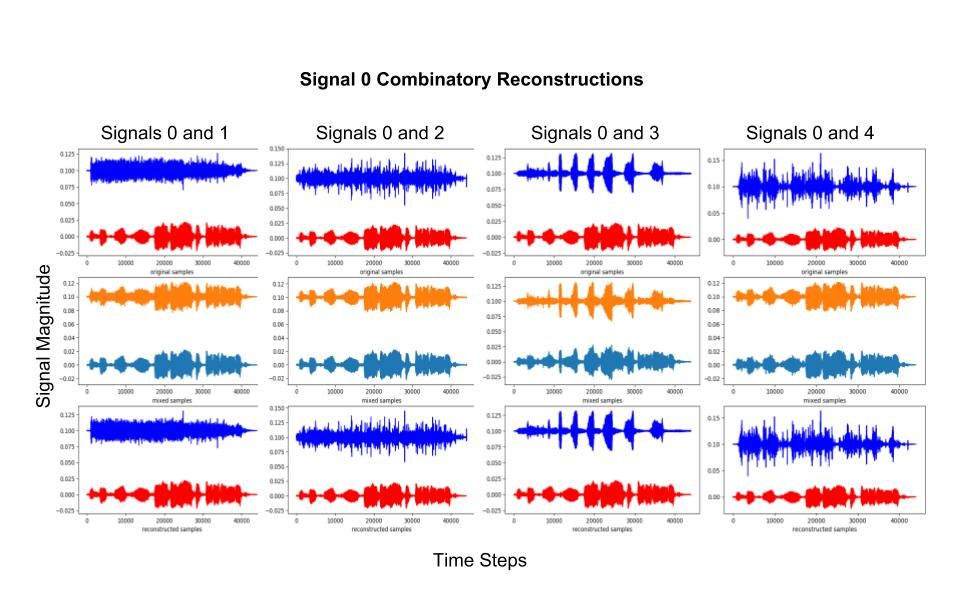
\includegraphics[width = 0.9\linewidth]{signals_0.jpg}
  \caption{Reconstruction of Signal 0 w.r.t Signals 1, 2, 3, and 4.}
\end{figure}
\FloatBarrier
\bigbreak
\noindent
In Figure 2 above, we can see that the mixture of Signals 0 and 1 and in the mixture of Signals 0 and 2, the blue signals (signal 1 and signal 2 respectively) are inverted in their reconstruction. This can be expected when using Independent Component Analysis. 

\begin{figure}[!htb] % replace 't' with 'b' to force it to be on the bottom
  \centering
  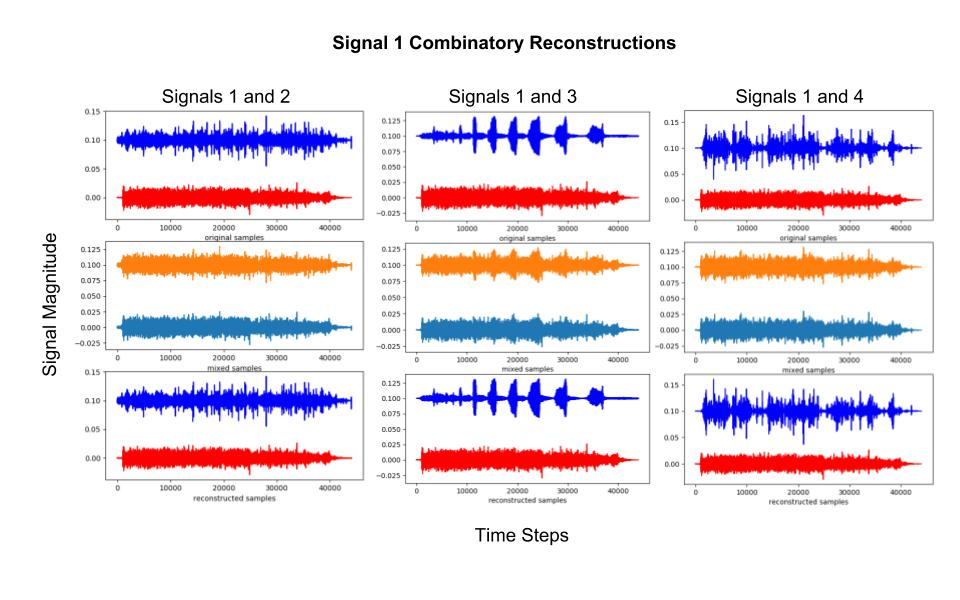
\includegraphics[width =0.7\linewidth]{signals_1.jpg}
  \caption{Reconstruction of Signal 1 w.r.t Signals 2, 3, and 4}
\end{figure}
\FloatBarrier
\begin{figure}[!htb] % replace 't' with 'b' to force it to be on the bottom
  \centering
  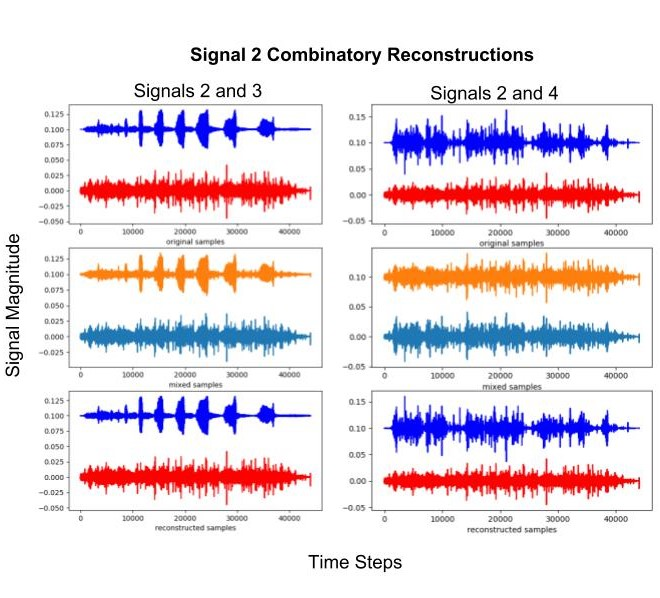
\includegraphics[width = 0.5\linewidth]{signals_2.jpg}
  \caption{Reconstruction of Signal 2 w.r.t 3 and 4}
\end{figure}
\FloatBarrier
\begin{figure}[!htb] % replace 't' with 'b' to force it to be on the bottom
  \centering
  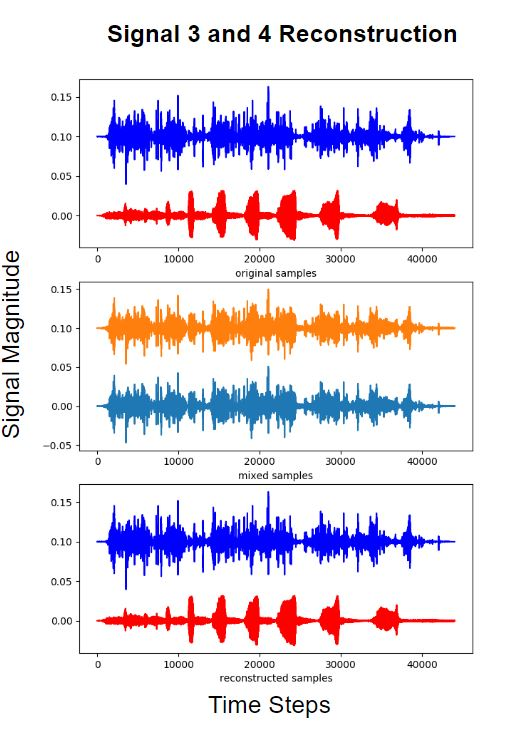
\includegraphics[width = 0.5\linewidth]{signals_3.JPG}
  \caption{Reconstruction of Signal 3 and 4}
\end{figure}
\FloatBarrier
\begin{table}[h!]
\centering
\begin{tabular}{ |p{3cm}||p{3cm}|p{3cm}|p{3cm}|  }
 \hline
 \multicolumn{3}{|c|}{Mean Squared Error of Mixed Signal Pairs} \\
 \hline
 Signal Pair& MSE First Signal & MSE Second Signal\\
 \hline
 Signal 0 and 1& 2.04609e-07& 9.06863e-08\\
 Signal 0 and 2& 1.40674e-09& 9.09086e-08\\
 Signal 0 and 3& 2.01816e-08& 9.25416e-09\\
 Signal 0 and 4& 4.31857e-11& 3.73872e-10\\
 Signal 1 and 2& 1.36941e-07& 1.35549e-07\\
 Signal 1 and 3& 2.46275e-10& 3.18763e-10\\
 Signal 1 and 4& 9.40809e-10& 9.09088e-08\\
 Signal 2 and 3& 2.67193e-09& 1.21463e-08\\
 Signal 2 and 4& 1.06596e-08& 9.08947e-08\\
 Signal 3 and 4& 4.81071e-12& 1.48309e-10\\
 \hline
\end{tabular}
\caption{Mean Squared Error of Signal Pairs}
\end{table}
\FloatBarrier
\noindent
It is important to note for Table 1 above that the mixing matrix A was not kept constant across measurements of accuracy. Therefore, it is difficult to judge which signal mixtures are easier to reconstruct over others. It is also important to note that the Mean Squared Error (MSE) accuracy measurement is a distance measurement. Given that the magnitudes of the signals are roughly [0, 0.5], the MSE will always look small (see Equation (18)). Generally speaking, the magnitudes of the errors (e-7 or smaller) are still far less than the magnitudes of the signals, thus the overall reconstruction using ICA and Gradient Descent is still very impressive.

\subsection{Multiple Source Signal Reconstruction}
The same metrics for signal identification, accuracy, and learning rate in the pair mixing in subsection 3.2 are used in this subsection. Figures 6-8 show BSS problems involving three mixed signals, four mixed signals, and five mixed signals respectively. Table 2 on page 11 summarizes the MSE accuracies from the experiments performed.

\begin{figure}[!htb] % replace 't' with 'b' to force it to be on the bottom
  \centering
  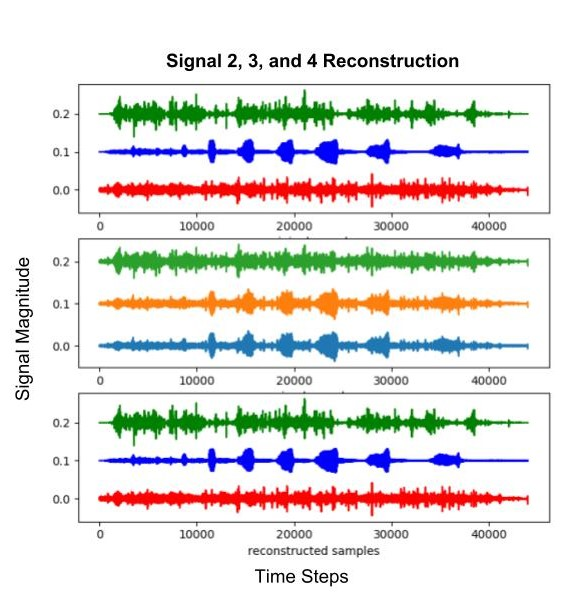
\includegraphics[width =0.7\linewidth]{sig_234.jpg}
  \caption{Reconstruction of Signals 2, 3, and 4}
\end{figure}
\FloatBarrier
\begin{figure}[!htb] % replace 't' with 'b' to force it to be on the bottom
  \centering
  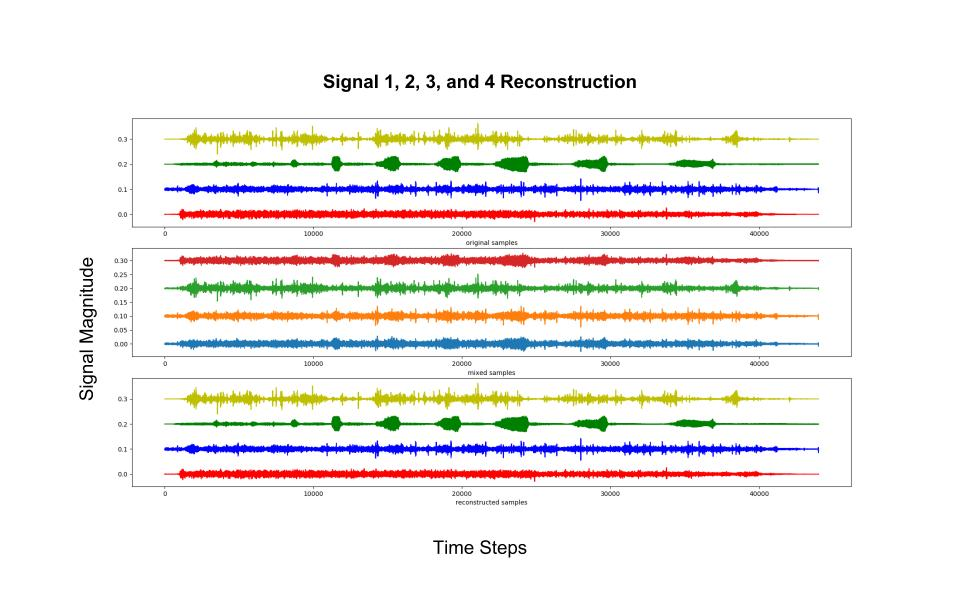
\includegraphics[width = \linewidth]{sig_1234.jpg}
  \caption{Reconstruction of Signals 1, 2, 3, and 4}
\end{figure}
\FloatBarrier
\begin{figure}[!htb] % replace 't' with 'b' to force it to be on the bottom
  \centering
  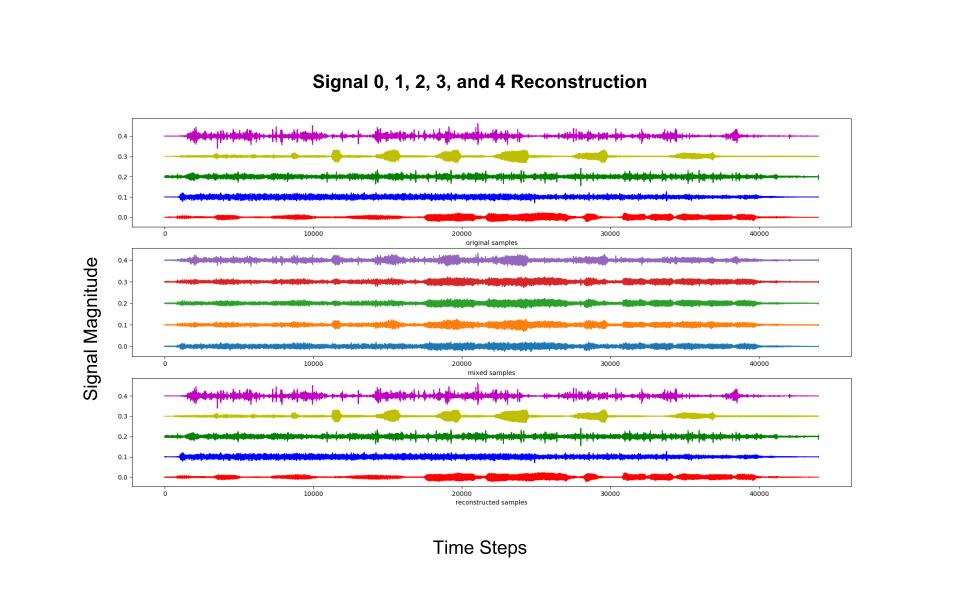
\includegraphics[width = \linewidth]{sig_01234.jpg}
  \caption{Reconstruction of Signals 0, 1, 2, 3, and 4}
\end{figure}
\FloatBarrier

\begin{table}[h!]
\centering
\resizebox{\textwidth}{!}{\begin{tabular}{ |c||c|c|c|c|c|  }
 \hline
 \multicolumn{5}{|c|}{Mean Squared Error of Mixed Signal Pairs} \\
 \hline
 Signal Pair& MSE First Signal & MSE Second Signal& MSE Third Signal & MSE Fourth Signal& MSE Fifth Signal\\
 \hline
 Signals 2,3, and 4 & 1.27534e-09& 1.48327e-09& 1.61670e-09& N/A & N/A\\
 Signals 1,2,3 and 4 & 2.82484e-08& 2.74507e-08& 4.96278e-09& 6.42436e-09 & N/A\\
 Signals 0,1,2,3 and 4& 1.50935e-09& 3.63869e-08& 2.96254e-08& 2.80287e-09& 2.58715e-09\\
 \hline
\end{tabular}}
\caption{Mean Squared Error of Signal Pairs}
\end{table}
\FloatBarrier
\noindent
Impressively, the mean squared errors for the multiple signal reconstruction stayed within the same order as the MSE for the pair signal measurements. However, the computational effort and ability to reach the optimum likelihood weights for W during gradient descent took much longer when adding additional signals to the mixing problem.

\subsection{Learning Rate's Effect on Accuracy (Mean Squared Error)}
In this section, the learning rate parameter is adjusted from \(10^{-2}\) to \(5\). It can be observed in Figure 9 below that the effect of learning rate on the mean squared error is minimal until reaching a learning rate of 3. Once this point is reached, an almost periodic triangle wave is produced. 
\begin{figure}[!htb] % replace 't' with 'b' to force it to be on the bottom
  \centering
  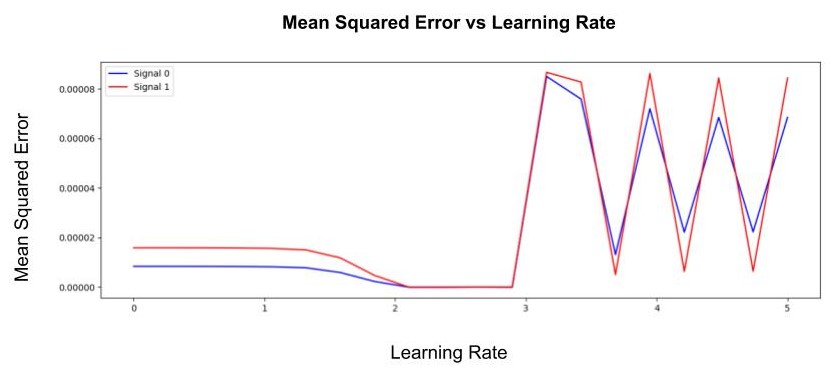
\includegraphics[width = \linewidth]{MSE_2.jpg}
  \caption{The Effect of the Learning Rate Parameter [0.001, 5] on Mean Squared Error}
\end{figure}
\FloatBarrier
\bigbreak
\noindent
This graph feature is an artifact of the artificial timer I set in my gradient descent loop. If my model does not converge after 10,000 iterations, my system will automatically return the signals in their current form. In some cases, this form is very close to maximum likelihood guess and produces a MSE minimum. In other cases, the form moves far away from the MSE minima as a result of iterating over a large step size (thus overshooting the maximum likelihood optimum.)
\bigbreak
\noindent
If the for loop time out did not exist, there is a reasonable chance that the system would not converge, making error calculations impossible to perform.
\subsection{Learning Rate's Effect on Convergence (Number of Update Iterations)}
The effect of the learning rate on convergence basically amounts to finding a "goldilocks" zone. In most stochastic gradient descent problems, the engineering trade off for selecting the learning rate involves minimizing the speed to converge by increasing the learning rate step size, but not massively over shooting the optima when getting closer to convergence. 
 
\begin{figure}[!htb] % replace 't' with 'b' to force it to be on the bottom
  \centering
  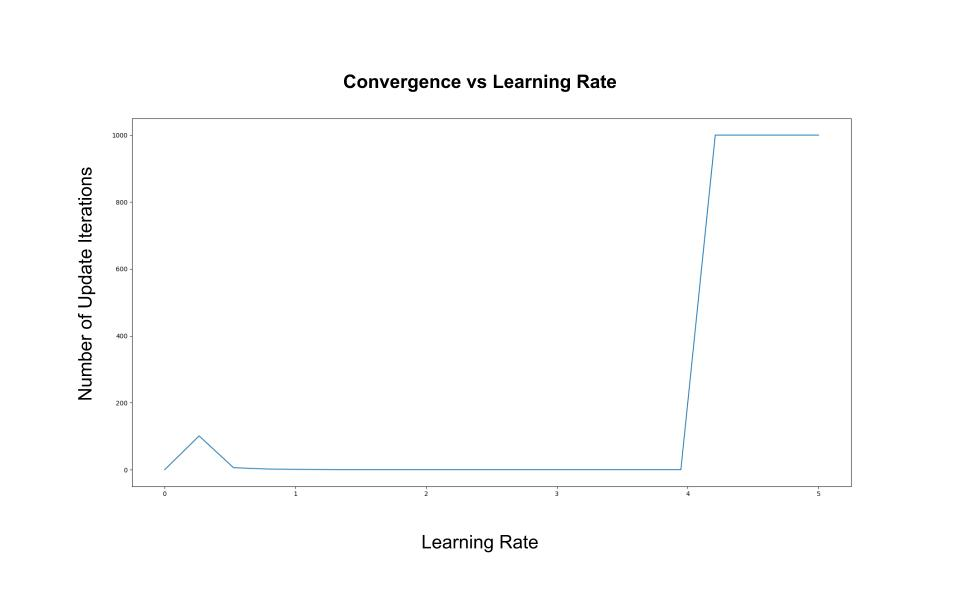
\includegraphics[width = \linewidth]{Conv.jpg}
  \caption{The Effect of the Learning Rate Parameter [0.001, 5] on Convergence}
\end{figure}
\FloatBarrier
\bigbreak
\noindent
In Figure 10 above, the "goldilocks" zone is around 0.5 to 3.5. In that range of values, it typically take 5-10 iterations for the system to converge. Once the learning rate surpasses 4, the system does not converge. The plateau at 1000 iterations is due to the for loop timer maxing out at 1000.
\section{Summary}
To solve the Blind Source Separation problem, Independent Component Analysis and Gradient Descent were used. On average, with a learning rate of 0.01 and a convergence condition of \(\left \| \Delta W \right \| < 0.0001\), the mean squared error of the reconstructed signals were on the order of \(10^{-8}\), thus indicating that the overall reconstruction was very good. 
\bigbreak
\noindent
By experimenting with the learning rate parameter, it was observed that it effects both the overall errors of signal reconstruction and convergence of the gradient descent algorithm. In both cases, an optimal zone of the learning parameter value exists. This is because a balance must be met between reaching the optimal zone quickly with large learning parameter step sizes versus not constantly overshooting the optimum after quickly getting close to it. It is common in stochastic gradient descent to address this issue by incorporating adaptive learning rates which scale down as you approach the optimum. 
\end{document}
              